\documentclass[12pt]{article}
\usepackage[utf8]{inputenc}
\usepackage[greek,english]{babel}
\usepackage{alphabeta}
\usepackage{fancyhdr}
\usepackage{listings}
\usepackage{mathtools}
\usepackage{xcolor}
\usepackage[backend=bibtex]{biblatex}
\usepackage{hyperref}
\usepackage[margin=0.5in]{geometry}
\usepackage{tikz}
\usetikzlibrary{automata, positioning, arrows}
\hypersetup{
	colorlinks=true,
	linktoc=all,
	linkcolor=black,
}
\lstset {
        basicstyle=\ttfamily,
        columns=fullflexible,
        breaklines=true,
        keepspaces=true,
	showstringspaces=false,
}
\tikzset{
	->,
	node distance=3cm,
}

\title{Θεωρία Υπολογισμού -- Εργασία 1}
\author{Χρήστος Μαργιώλης -- 19390133}
\date{Νοέμβριος 2025}

\begin{document}

\begin{titlepage}
        \maketitle
        \begin{figure}[t!]
        \begin{center}
        
\includegraphics[scale=0.3]{./res/uniwalogo.png} \\
        \Large
        \textbf{Πανεπιστήμιο Δυτικής Αττικής} \\
        \large
        Τμήμα Μηχανικών Πληροφορικής και Ηλεκτρονικών Υπολογιστών
        \end{center}
        \end{figure}
\end{titlepage}

\section{Άσκηση 1}

Οι κανονικές εκφράσεις $R_1$ και $R_2$ περιγράφουν τις εξής γλώσσες:

\[
	\mathcal{L}(R_1) =
	\mathcal{L}((a^*b^*)^*) =
	(\mathcal{L}(a^*b^*))^* =
	(\{a,b\})^* =
	\{a,b\}^*
\]

\[
	\mathcal{L}(R_2) =
	\mathcal{L}((a \cup b)^*) =
	(\mathcal{L}(a) \cup \mathcal{L}(b))^* =
	(\{a\} \cup \{b\})^* =
	\{a,b\}^*
\]

Επομένως, οι ΚΕ περιγράφουν την ίδια γλώσσα.

\section{Άσκηση 2}

\begin{center}
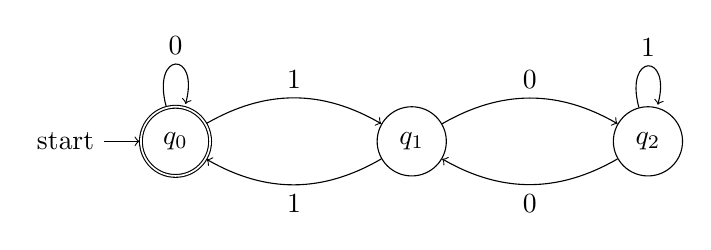
\begin{tikzpicture}
	\node[state, accepting, initial] (q0) {$q_0$};
	\node[state, right of=q0] (q1) {$q_1$};
	\node[state, right of=q1] (q2) {$q_2$};

	\draw (q0) edge[loop above] node{0} (q0);
	\draw (q0) edge[bend left, above] node{1} (q1);
	\draw (q1) edge[bend left, below] node{1} (q0);
	\draw (q1) edge[bend left, above] node{0} (q2);
	\draw (q2) edge[bend left, below] node{0} (q1);
	\draw (q2) edge[loop above] node{1} (q2);
\end{tikzpicture}
\end{center}

Τo ΝΠΑ ορίζεται ως $Μ(Κ,Σ,s,F,δ)$, όπου $K = \{q_0,q_1,q_2\}$, $Σ = \{0,1\}$,
$s = q_0$, $F = q_0$ και $δ$:

\begin{center}
\begin{tabular}{ccc}
	$q$ & $σ$ & $δ(q, σ)$ \\
	\hline
	$q_0$ & 0 & $q_0$ \\
	$q_0$ & 1 & $q_1$ \\
	$q_1$ & 0 & $q_2$ \\
	$q_1$ & 1 & $q_0$ \\
	$q_2$ & 0 & $q_1$ \\
	$q_2$ & 1 & $q_2$ \\
\end{tabular}
\end{center}

Ο λόγος που έχουμε 3 καταστάσεις είναι διότι η πράξη $x \mod 3$ έχει 3 πιθανά
αποτέλεσματα: $\{0, 1, 2\}$. Μπορούμε να επαληθεύσουμε το παραπάνω ΝΠΑ με
μερικά παραδείγματα. Προκειμένου ένας αριθμός να είναι πολλαπλάσιο του 3,
πρέπει η τελευταία κατάσταση που θα επανέλθουμε να είναι η $F= q_0$. Ας
υποθέσουμε την εκτέλεση του ΝΠΑ με είσοδο το 1001 (9):

\begin{itemize}
	\item $q_0 = 1 \mod 3 = 1 \rightarrow q_1$
	\item $q_1 = 0 \mod 3 = 0 \rightarrow q_2$
	\item $q_2 = 0 \mod 3 = 0 \rightarrow q_1$
	\item $q_1 = 1 \mod 3 = 1 \rightarrow q_0$
\end{itemize}

Επιστρέψαμε στην κατάσταση $q_0$ μετά την ανάλυση όλων των ψηφίων, οπότε ο
αριθμός είναι πολλαπλάσιο του 3, το οποίο ισχύει, διότι $9 \mod 3 = 0$.

Αντιθέτως, ας δώσουμε ως είσοδο ένα μη-πολλαπλάσιο του 3, το 10 (2):

\begin{itemize}
	\item $q_0 = 1 \mod 3 = 1 \rightarrow q_1$
	\item $q_1 = 0 \mod 3 = 0 \rightarrow q_2$
\end{itemize}

Σε αυτήν την περίπτωση τελειώσαμε στην κατάσταση $q_2$, οπότε το 10 (2) δεν
είναι πολλαπλάσιο του 3, το οποίο επιβεβαιώνεται από το $2 \mod 3 = 2$.

\section{Άσκηση 4}

\begin{center}
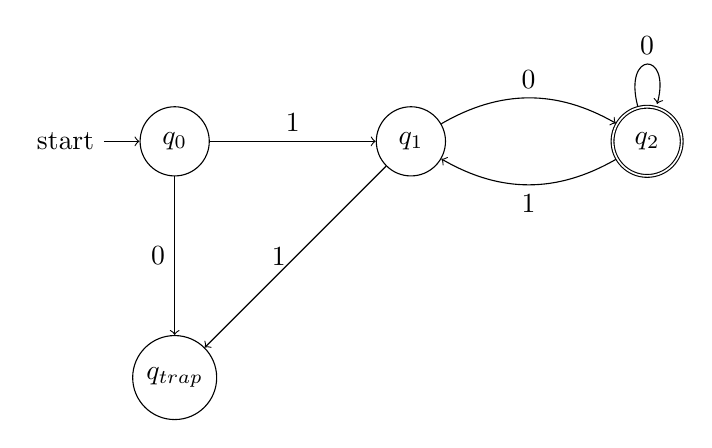
\begin{tikzpicture}
	\node[state, initial] (q0) {$q_0$};
	\node[state, below of=q0] (qtrap) {$q_{trap}$};
	\node[state, right of=q0] (q1) {$q_1$};
	\node[state, accepting, right of=q1] (q2) {$q_2$};

	\draw (q0) edge[above] node{1} (q1);
	\draw (q0) edge[left] node{0} (qtrap);
	\draw (q1) edge[left] node{1} (qtrap);
	\draw (q1) edge[bend left, above] node{0} (q2);
	\draw (q2) edge[bend left, below] node{1} (q1);
	\draw (q2) edge[loop above] node{0} (q2);
\end{tikzpicture}
\end{center}

Τo ΝΑ ορίζεται ως $Μ(Κ,Σ,s,F,δ)$, όπου $K = \{q_0,q_1,q_2, q_{trap}\}$, $Σ = \{0,1\}$,
$s = q_0$, $F = q_2$ και $δ$:

\begin{center}
\begin{tabular}{ccc}
	$q$ & $σ$ & $δ(q, σ)$ \\
	\hline
	$q_0$ & 0 & $q_{trap}$ \\
	$q_0$ & 1 & $q_1$ \\
	$q_1$ & 0 & $q_2$ \\
	$q_1$ & 1 & $q_{trap}$ \\
	$q_2$ & 0 & $q_2$ \\
	$q_2$ & 1 & $q_1$ \\
\end{tabular}
\end{center}

\section{Άσκηση 6}

\[
	\epsilon|(b^*(ab)^*)
\]

Η παραπάνω ΚΕ είναι επαρκής διότι αρχικά δέχεται την κενή συμβολοσειρά
$\epsilon$. Επίσης, εφόσον υπάρχει ο περιορισμός ότι κάθε \textit{a} πρέπει
οπωσδήποτε να ακολουθείται από \textit{b}, τότε χρειαζόμαστε την ΚΕ $(ab)^*$.
Έπειτα, μπορούμε να έχουμε 0 ή παραπάνω \textit{b}, οπότε αυτό καλύπτεται από
την ΚΕ $b^*$.

\end{document}
